\documentclass[10pt]{beamer}

% ---- Packages ----

\usepackage[utf8]{inputenc}
\usepackage[T1]{fontenc}
\usepackage[spanish]{babel}
\usepackage{epsfig}
\usepackage{graphics}
\usepackage{tabularx}
\usepackage{listings}
\usepackage{noto}
\usepackage{eurosym}
\usepackage{epsfig}
\usepackage{amssymb}
\usepackage{amsmath}
\usepackage{xcolor}

% ---- Configuration ----

\usetheme{Madrid}
\useinnertheme{circles}
\usenavigationsymbolstemplate{}
\setbeamertemplate{blocks}[rounded]

\definecolor{UDCpink}{RGB}{214,30,140}
\definecolor{UDCgray}{RGB}{100,100,100}

\usecolortheme[named=UDCpink]{structure}

\makeatletter
\setbeamertemplate{title page}
{
	\vbox{}
	\vspace{0.25em}
	\begin{centering}
		{\usebeamercolor[fg]{titlegraphic}\inserttitlegraphic\par}
		\vspace{1em}
		\begin{beamercolorbox}[sep=8pt,center,rounded=true]{title}
			\usebeamerfont{title}\inserttitle\par%
			\ifx\insertsubtitle\@empty%
			\else%
			\vspace{0.25em}
			{\usebeamerfont{subtitle}\usebeamercolor[fg]{subtitle}\insertsubtitle\par}%
			\fi%     
		\end{beamercolorbox}%
		\vfill
		\begin{beamercolorbox}[sep=8pt,center]{author}
			\usebeamerfont{author}\insertauthor
		\end{beamercolorbox}
		\begin{beamercolorbox}[sep=8pt,center]{institute}
			\usebeamerfont{institute}\insertinstitute
		\end{beamercolorbox}
		\begin{beamercolorbox}[sep=8pt,right]{date}
			\itshape\usebeamerfont{date}\insertdate
		\end{beamercolorbox}
	\end{centering}
	\vspace{0.25em}
}
\makeatother

\lstdefinestyle{myLuastyle}
{
	language         = {[5.2]Lua},
	commentstyle=\color{green},
	keywordstyle=\color{blue}, 
	basicstyle = \ttfamily \color{black} \footnotesize
}

\lstset{style=myLuastyle}

% ---- Document ----

\title[Generación mediante ASP]{Generación de Escenarios de un Videojuego 2D mediante Programación Lógica}
\author[Rafael Alcalde Azpiazu]{\large Rafael Alcalde Azpiazu}
\institute[UDC] % (optional)
{
	\normalsize
	Grado en Ingeniería Informática \\
	Mención en Computación \\
	\vspace{1em}
	Proyecto clásico de Ingeniería \\
	Facultad de Informática \\
	\vspace{1em}
	Director: José Pedro Cabalar Fernández  \\
}
\date[]{A Coruña, \today}
\titlegraphic{
\includegraphics[height=2em]{images/logo.png}}

\begin{document}
	
	\begin{frame}
		\titlepage
	\end{frame}

	\section{Motivación}
	\begin{frame}
	\frametitle{Motivación}

	\begin{itemize}
		\item<1-> La \textcolor{UDCpink}{industria del videojuego} constituye un sector económico cada vez más relevante.
		
		\vspace{0.5em}
		
		\begin{itemize}
			\item<2-> (En \$) Minecraft: 2500 millones, Fornite: 1000 millones, Destiny: 500 millones.
		\end{itemize}
	
		\vspace{1em}
		
		\item<3-> Ha activado avances tecnológicos, p. ej. el uso de la {Inteligencia Artificial}, uno de los campos que más ha contribuido.
		
		\vspace{0.5em}
		
		\begin{itemize}
			\item<4-> Diseño de enemigos inteligentes mediante programación evolutiva (p. ej. No Man's Sky).
			
			\vspace{0.5em}
			
			\item<5-> \textcolor{UDCpink}{Diseño del entorno}. Existen dos aproximaciones:
			
			\vspace{0.5em}
			
			\begin{itemize}
				\item<5-> Generación procedimental. La más usada.
				
				\vspace{0.5em}
				
				\item<7-> \textcolor{UDCpink}{Generación declarativa} $\Leftarrow$.
			\end{itemize}
		\end{itemize}
	\end{itemize}
\end{frame}

\begin{frame}
	\frametitle{Diseño de entornos}
	
	\begin{itemize}
		\item<1-> \textcolor{UDCpink}{Generación procedimental}: se basa en un algoritmo o técnica ya predefinida.
		
		\vspace{1em}
		
		\begin{enumerate}
			\item<2-> Algoritmo ad-hoc.
			
			\vspace{0.5em}
			
			\item<3-> Programación evolutiva.
			
			\vspace{0.5em}
			
			\item<4-> Expresiones matemáticas.
		\end{enumerate}
	\end{itemize}
	
	\vspace{1em}
	
	\pause[5]
	
	\begin{block}{\normalsize Problemática}
		\vspace{1em}
		Para \textcolor{UDCpink}{influir} en el resultado de la generación se necesita \textcolor{UDCpink}{reprogramar} el algoritmo generador para adaptarlo a los criterios.
		\vspace{1em}
	\end{block}
\end{frame}

\begin{frame}
\frametitle{Diseño de entornos}

	\begin{itemize}
		\item<1-> \textcolor{UDCpink}{Generación declarativa}: existe una representación formal del entorno, p. ej. mediante \textcolor{UDCpink}{programación lógica}.
		
		\vspace{1em}
		
		\item<2-> La técnica es \textcolor{UDCpink}{independiente} del algoritmo de búsqueda usado para obtener las posibles soluciones.
		
		\vspace{1em}
		
		\item<3-> Un caso concreto de programación lógica es \textcolor{UDCpink}{\textit{Answer Set Programming}}.
		
		\vspace{0.5em}
		
		\begin{itemize}
			\item<4-> \textit{Answer Set Programming for Procedural Content Generation: A Design Space Approach} \textcolor{UDCpink}{[Smith et al, 11]} (ASP + Warzone 2100).
			
			\vspace{0.5em}
			
			\item<5-> En este proyecto: \textcolor{UDCpink}{ASP + Freeciv} $\Leftarrow$.
		\end{itemize}
	\end{itemize}

\end{frame}
	\begin{frame}
	\frametitle{Freeciv}

	\begin{columns}
		
		\column{0.6\textwidth}
		\begin{itemize}
			\item<1-> Versión \textcolor{UDCpink}{\textit{open source}} y \textcolor{UDCpink}{gratuita} de Sid Meier's Civilization creado en la universidad de Aarhus.
			
			\vspace{1em}
			
			\item<2-> Juego de \textcolor{UDCpink}{estrategia por turnos}.
			
			\vspace{1em}
			
			\item<3-> El jugador controla a un \textcolor{UDCpink}{grupo de colonos}, comienza en el año \textcolor{UDCpink}{4000 A.C}.
			
			\vspace{1em}
			
			\item<4-> El objetivo final es crear una \textcolor{UDCpink}{gran civilización}. Para ello existen \textcolor{UDCpink}{5 formas} de finalizar el juego:
			
			\vspace{0.5em}
			
			\begin{itemize}
				\item Victoria por \textcolor{UDCpink}{dominación}, \textcolor{UDCpink}{científica}, \textcolor{UDCpink}{religión}, \textcolor{UDCpink}{cultural} o \textcolor{UDCpink}{por puntuación}.
			\end{itemize}
		\end{itemize}

		\column{0.4\textwidth}
		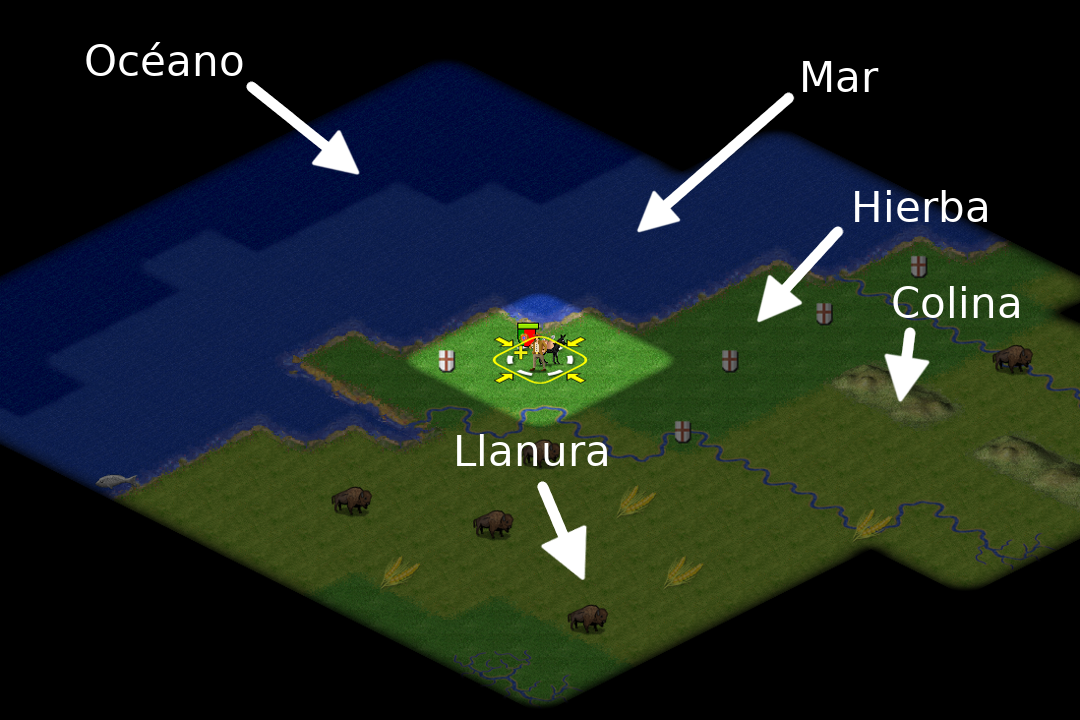
\includegraphics[width=\textwidth]{images/freeciv-example.png}
	\end{columns}

\end{frame}

\begin{frame}
\frametitle{Tipos de terrenos en Freeciv}

\begin{itemize}
	\item Hay \textcolor{UDCpink}{12 tipos de terreno}, con posibles bonificaciones.
\end{itemize}

\vspace{0.5em}

\centering
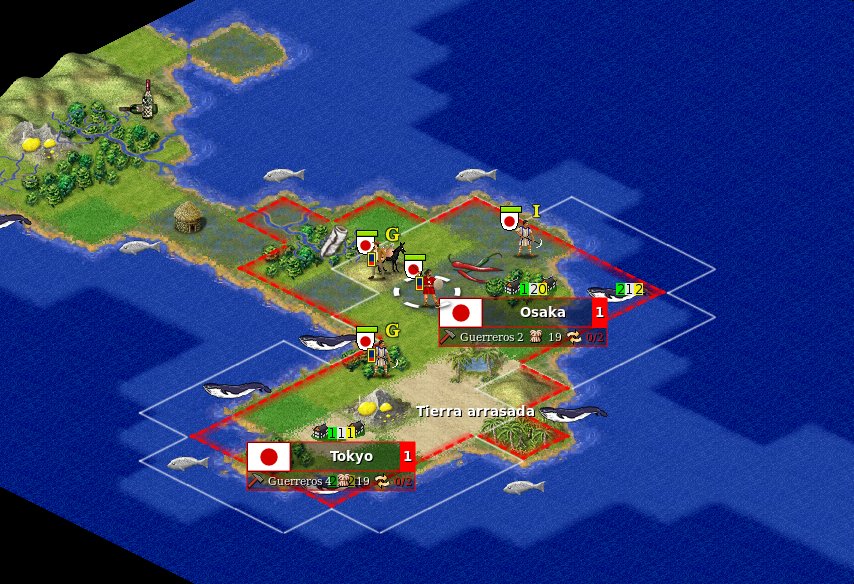
\includegraphics[width=0.8\textwidth]{images/ejemplo-partida.png}
\end{frame}


\begin{frame}
\frametitle{Objetivos del proyecto}

Para este proyecto:

\vspace{1em}

\begin{itemize}
	\item<1-> Se definirá un \textcolor{UDCpink}{modelo declarativo} del escenario para Freeciv usando \textcolor{UDCpink}{\itshape Answer Set Programming}.
	
	\vspace{1em}
	
	\item<2-> Se construirá una pequeña \textcolor{UDCpink}{herramienta gráfica} con la que manipular el escenario.
	
	\vspace{1em}
	
	\item<3-> Eficiencia: reducir o podar el número de combinaciones posibles.
\end{itemize}

\end{frame}

	
	\begin{frame}
	\frametitle{Índice}
		\tableofcontents
	\end{frame}
	
	\AtBeginSection[]
	{
	\begin{frame}
	\frametitle{Índice}
	\tableofcontents[currentsection]
	\end{frame}
	}
	
	\section{Answer Set Programming}
	\begin{frame}
	\frametitle{Answer Set Programming}

	\begin{itemize}
		\item<1-> Paradigma enfocado a la \textcolor{UDCpink}{resolución declarativa} de problemas con complejidad \textcolor{UDCpink}{\textit{NP-hard}}.
		
		\vspace{0.5em}
		
		\item<2-> Combina un \textcolor{UDCpink}{lenguaje simple} con el que modelar problemas lógicos y \textcolor{UDCpink}{herramientas de alto rendimiento}.
	\end{itemize}

	\vspace{1em}
	
	\pause[3]
	
	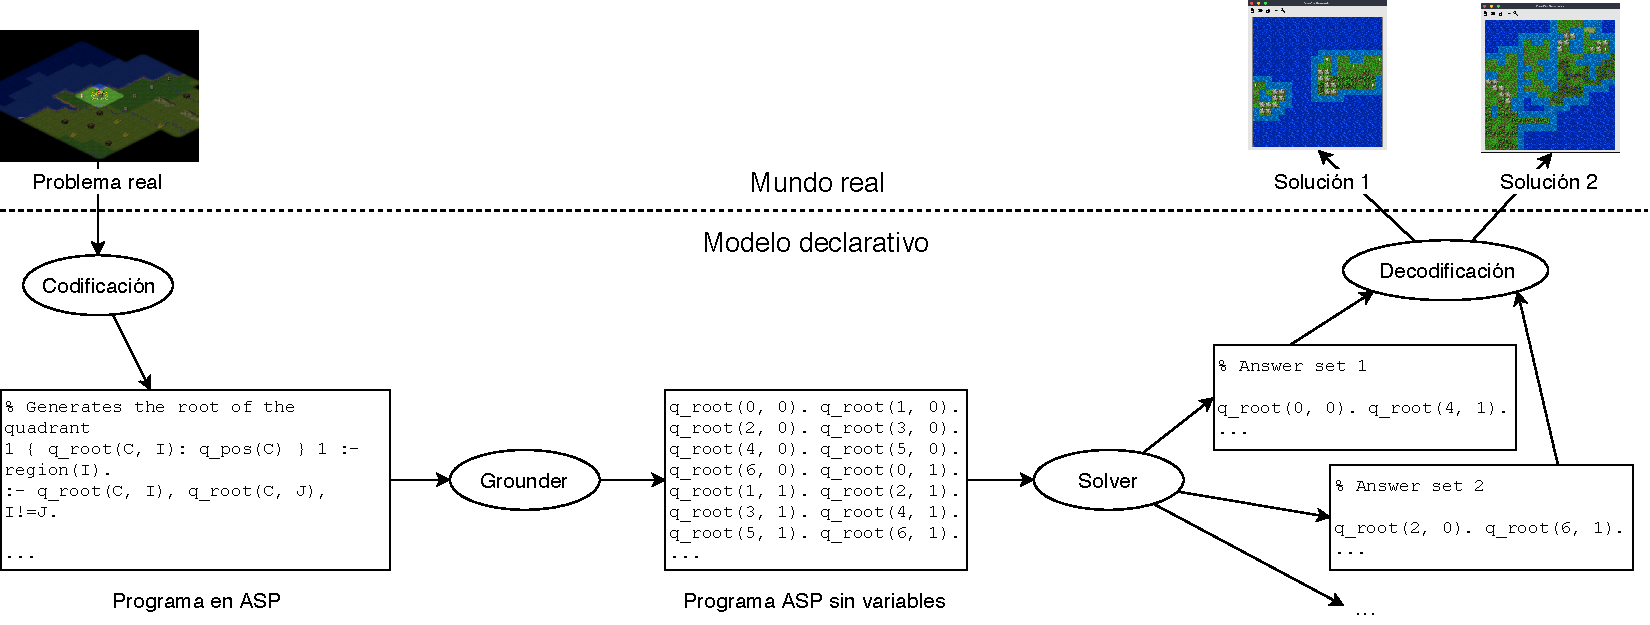
\includegraphics[width=\textwidth]{images/funcionamiento-asp.pdf}
	
\end{frame}

\begin{frame}
	\frametitle{Ejemplo de reglas lógicas}
	
	\begin{block}{Generación del cuadrantes}
	\vspace{1em}
	\hspace{2em}\texttt{1 \{ q\_root(C, I): q\_pos(C) \} 1 :- region(I).}
	
	\hspace{2em}\texttt{:- q\_root(C, I), q\_root(C, J), I!=J.}
	
	\vspace{2em}
	
	\hspace{2em}\texttt{q\_reached(C, I) :- q\_root(C, I).} 
	
	\hspace{2em}\texttt{\{q\_reached(C, I)\} :- q\_reached(D, I), region(I),}
	
	\hspace{4em}\texttt{not existsanother(I, C), q\_adj(D, C).}
	
	\hspace{2em}\texttt{existsanother(I, C) :- q\_reached(C, J), region(J),}
	
	\hspace{4em}\texttt{region(I), J!=I.}
	\vspace{1em}
	\end{block}
	
\end{frame}
	
	\section{Demostración}
	
	\section{Trabajo desarrollado}
	\subsection{First approach}
\begin{frame}
\frametitle{First approach}

\begin{columns}
	\column{0.25\textwidth}
	\centering 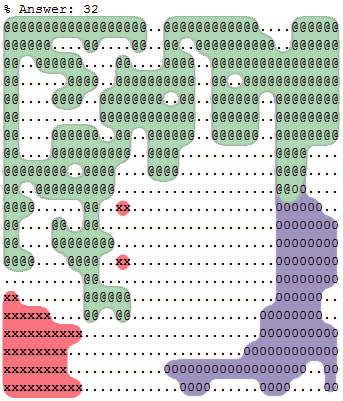
\includegraphics[width=0.7\textwidth]{images/adam.png}
	
	\column{0.75\textwidth}
	\begin{itemize}
		\item<1-> \textit{Answer Set Programming for Procedural Content Generation: A Design Space Approach} \textcolor{UDCpink}{[Smith \& Mateas 11]}
		\item<2-> This approximation creates a single solid island.
		\item<3-> But I need more that one island.
	\end{itemize} 
\end{columns}
	
\end{frame}

\begin{frame}
\frametitle{First approach}

\begin{itemize}
	\item<1-> I created a starting point for generate an island.
	\item<2-> I expanded this points with adjacency rules.
	\item<3-> I added the restriction rules to the adjacent islands not stick together.
	\item<4-> \textcolor{UDCpink}{Problem:} This approach was inefficient with large maps.
\end{itemize}

\end{frame}

\subsection{Second approach}

\begin{frame}
\frametitle{Second approach}

\begin{itemize}
	\item<1-> I divided the map in regions.
	\item<2-> One region is a single island.
	\item<3-> I used the Lua build-in module clingo to call only one region generation.
	\item<4-> Once this work, I generated all the regions with build-in module.
	\item<5-> Finally I added the restriction rules to the regions not stick together.
\end{itemize}

\end{frame}

\subsection{Related work}

\begin{frame}
\frametitle{Related work}

\begin{itemize}
	\item<1-> Add user restrictions to the generation.
	\item<2-> Add all types of terrain.
	\item<3-> Generate player starting points.
	\item<4-> Add a exporter to Freeciv.
\end{itemize}

\end{frame}
	\begin{frame}
\frametitle{Uso de la biblioteca de Clingo}

\begin{itemize}
	\item<1-> Permite embeber código en Lua (por defecto) o en Python (recompilándolo).
	
	\vspace{0.5em}
	
	\item<2-> Los dos lenguajes comparten la interfaz de funciones, variables, 
	métodos, etc.
	
	\vspace{0.5em}
	
	\item<3-> Para este proyecto se ha usado \textcolor{UDCpink}{Lua}.
\end{itemize}

\vspace{0.5em}

\pause[4]

\centering
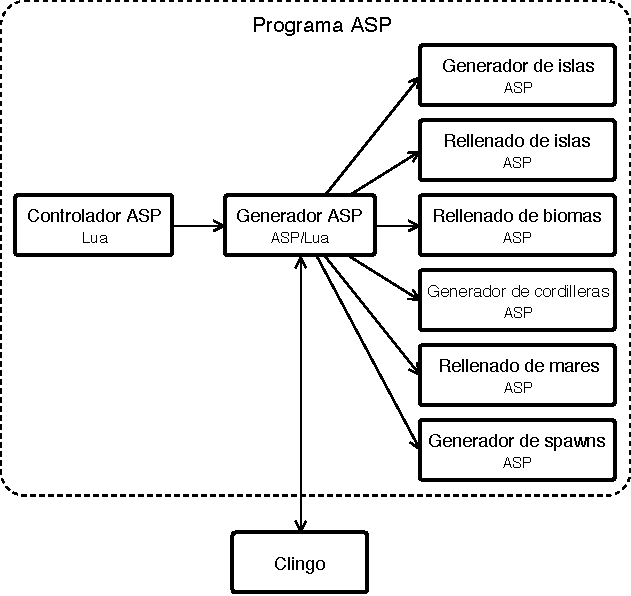
\includegraphics[width=0.4\textwidth]{images/arquitectura-final.pdf}
\end{frame}
	\begin{frame}
\frametitle{Arquitectura del sistema}

\begin{itemize}
	\item<1-> \textcolor{UDCpink}{\itshape Front-end}: Creado en \textcolor{UDCpink}{LÖVE}, usa un modelo MVC que usa una interfaz gráfica en modo inmediato.
	
	\vspace{0.5em}
	
	\item<2-> \textcolor{UDCpink}{\itshape Back-end}: Creado en \textcolor{UDCpink}{Lua} (con API de clingo) y \textcolor{UDCpink}{ASP}, usa un modelo en \textit{pipeline}.
\end{itemize}

\pause[3]

\begin{center}
	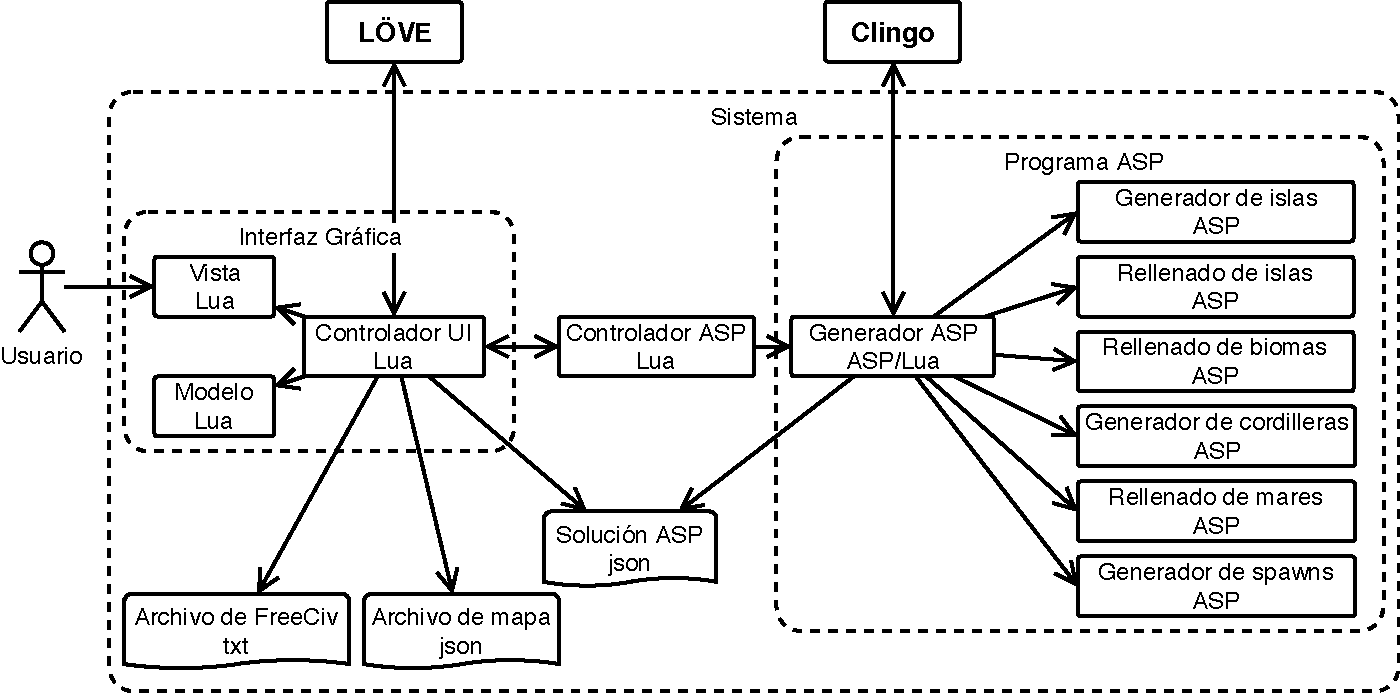
\includegraphics[width=.95\textwidth]{images/arquitectura-completa.pdf}
\end{center}

\end{frame}

\begin{frame}
\frametitle{Proceso de ingeniería}

\begin{itemize}
	\item<1-> Metodología: \textcolor{UDCpink}{desarrollo iterativo incremental y evolutivo}.
	
	\vspace{0.5em}
	
	\item<2-> Se ha usado herramientas de \textcolor{UDCpink}{uso libre y gratuitas} para el desarrollo del proyecto.
	
	\vspace{0.5em}
	
	\item<3-> El coste total del proyecto asciende a \textcolor{UDCpink}{\EUR{3720.00}}.
	
	\vspace{0.5em}	
\end{itemize}

\pause[4]

\centering
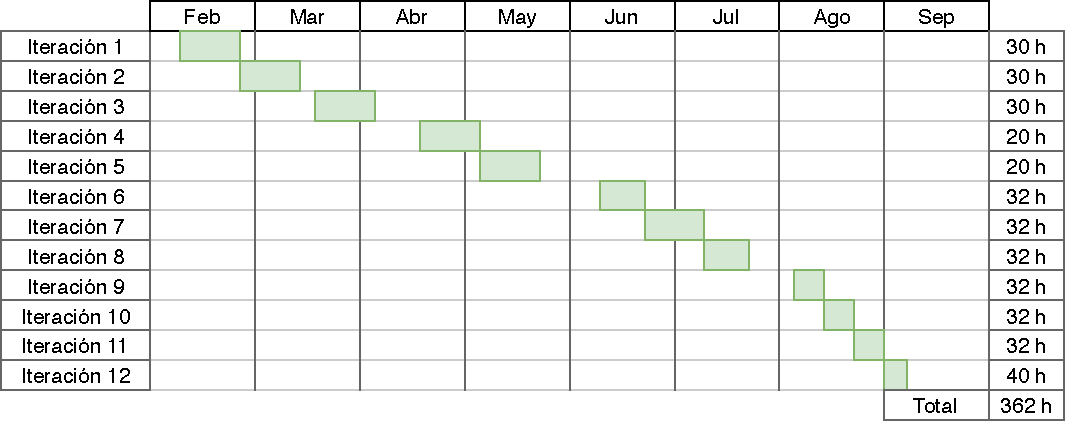
\includegraphics[width=\textwidth]{images/gantt.pdf}

\end{frame}

	\section{Evaluación}
	En este capítulo se analizará los resultados obtenidos en el proceso de evaluación del sistema. Para la planificación de las pruebas se ha optado por el uso de una herramienta de integración continua en donde se corren tanto pruebas de unidad a las partes del modelo de la interfaz gráfica, así como a los distintos módulos de los programas lógicos. \\

Además se ha usado un programa escrito en Lua para la ejecución de pruebas de rendimiento o \textit{benchmarks} el cual solo usa el módulo clingo para evitar el uso de la interfaz gráfica. En todas estas pruebas se ha añadido a las pruebas la restricción de que el cómputo del mapa solo puede durar como máximo cinco minutos, matando el proceso en caso de superar este tiempo y pasando a la siguiente prueba. Con esto podemos indicar cuales son las configuraciones que dan una experiencia pobre al usuario. \\

A continuación se describen los resultados obtenidos de estas pruebas de rendimiento con distintos parámetros. \\

\section{Tamaño de los mapas}

Estas pruebas se han realizado usando distintos tamaños de mapas cuadrados, dejando el resto de variables con valores por defecto (cantidad de tierra y de biomas al 20\%, tamaño de las cordilleras en 2 casillas, longitud de cordilleras en 3 casillas, 2 jugadores y 2 casillas de distancia mínima entre jugadores). \\

Debido a que el módulo pide el número de cuadrantes y el tamaño en casillas de un cuadrante, se han realizado las pruebas calculando primero el tamaño total del mapa y con esto se ha obtenido tres números números:

\begin{align}
	islands &= \lfloor \sqrt{size} - 1 \rfloor \\
	n_1 | size, & \text{ en donde } n_1 > islands. \\
	n_2 &= size / n_1
\end{align}

Con esto se procede a obtener el número de cuadrantes y el tamaño del cuadrante mediante:

\begin{align}
	q_{num} &= min(n_1, n_2) \\
	q_{size} &= max(n_1, n_2) \\
\end{align}

\begin{table}[!h]
	\begin{tabularx}{\textwidth}{ X X X X X X }
		\bfseries{Tamaño} & \bfseries{Islas} & $\mathbf{q_{num}}$ & $\mathbf{q_{size}}$ & \bfseries{Total} & \bfseries{Ejecución} \\
		\hline
		10 x 10 & 2 & 2 & 5 & 6 s & 117 ms \\
		15 x 15 & 2 & 3 & 5 & 17 s & 145 ms \\
		20 x 20 & 3 & 4 & 5 & 88 s & 296 ms \\
		25 x 25 & 4 & 5 & 5 & 200 s & 675 ms \\
		30 x 30 & 4 & 5 & 6 & 1137 s & 731 ms \\
		35 x 35* & 4 & 5 & 7 & - & - \\
		40 x 40 & 5 & 5 & 8 & 1791 s & 1050 ms \\
		45 x 45 & 5 & 5 & 9 & 4627 s & 1047 ms \\
		\hline
	\end{tabularx}
	\begin{tablenotes}
		\item[1] Las filas indicadas con - se refieren a las pruebas en donde una ejecución no se han podido completan en menos de 5 minutos.
	\end{tablenotes}
	\caption{Resultado del \textit{benchmark} con diferentes tamaños de mapa.}\label{table:mapresult}
\end{table}

\begin{figure}[!h]
	\centering
	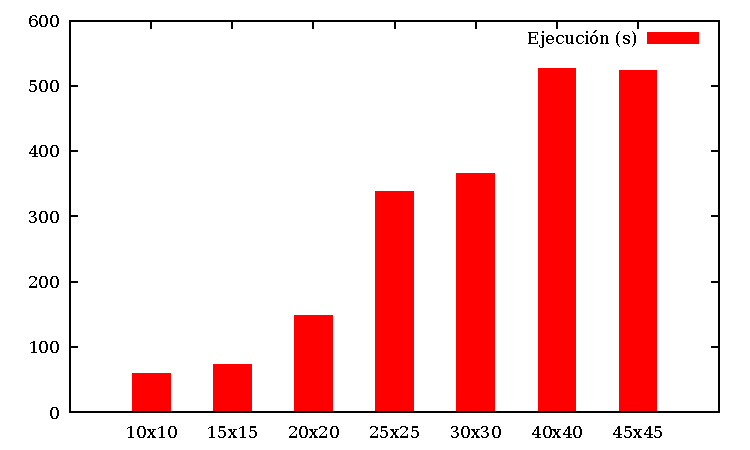
\includegraphics[width=.8\textwidth]{tables/map-size.pdf}
	\caption{Tiempos del \textit{benchmark} con diferentes tamaños de mapa.}\label{fig:mapresult}
\end{figure}

Con esto nos aseguramos de que cada uno de los módulos tengan porciones parecidas para computar. En la Tabla \ref{table:mapresult} podemos ver los resultados de la realización de esta prueba de rendimiento ejecutando 25 ejecuciones cada una de las medidas, en donde se recoge el tiempo total de todas las ejecuciones, el tiempo total que ha usado clingo para obtener una solución y el tiempo medio de una ejecución. Por otra parte en la Figura \ref{fig:mapresult} podemos ver una comparativa entre el tiempo medio entre ejecuciones y el tiempo medido arrojado por clingo. \\

Como se puede observar, el tiempo de ejecución sigue una tendencia casi exponencial, haciendo que a partir de mapas de 45x45 celdas en ningún momento la ejecución tarde menos de 5 minutos. Aún así, hay que destacar un caso concreto, ya que la prueba de un mapa de 35x35 celdas con los valores propuestos se realiza en más de 5 minutos, cosa que tanto en las pruebas anteriores como en las siguientes no ocurre. Esto puede deberse a que el mapa para esta prueba no esté bien repartido para los distintos módulos.  

\section{Porcentajes de tierra y biomas}
\label{sec:pruebatierrabiomas}

Para la primera parte de la prueba se ha usado distintos porcentajes de tierra, usando la cantidad de islas y los parámetros de cantidad y tamaño de los cuadrantes para mapas de 25x25 celdas de la prueba anterior y dejando el resto de variables con valores por defecto (cantidad de biomas al 20\%, tamaño de las cordilleras en 2 casillas, longitud de cordilleras en 3 casillas, 2 jugadores y 2 casillas de distancia mínima entre jugadores). \\

\begin{table}[!h]
	\centering
	\begin{tabular}{ c c c }
		\bfseries{Porcentaje} & \bfseries{Total} & \bfseries{Ejecución} \\
		\hline
		10\% & 174 s & 6,96 s \\
		15\% & 178 s & 7,12 s \\
		20\% & 178 s & 7,12 s \\
		25\% & 179 s & 7,16 s \\
		30\% & 181 s & 7,24 s \\
		35\% & 178 s & 7,12 s \\
		40\% & 179 s & 7,16 s \\
		45\% & 178 s & 7,12 s \\
		50\% & 181 s & 7,24 s \\
		55\% & 179 s & 7,16 s \\
		60\% & 178 s & 7,12 s \\
		65\% & 179 s & 7,16 s \\
		70\% & 178 s & 7,12 s \\
		75\% & 180 s & 7,20 s \\
		80\% & 180 s & 7,20 s \\
		\hline
	\end{tabular}
	\caption{Resultado del \textit{benchmark} con diferentes porcentajes de tierra.}\label{table:landresult}
\end{table}

\begin{figure}[!h]
	\centering
	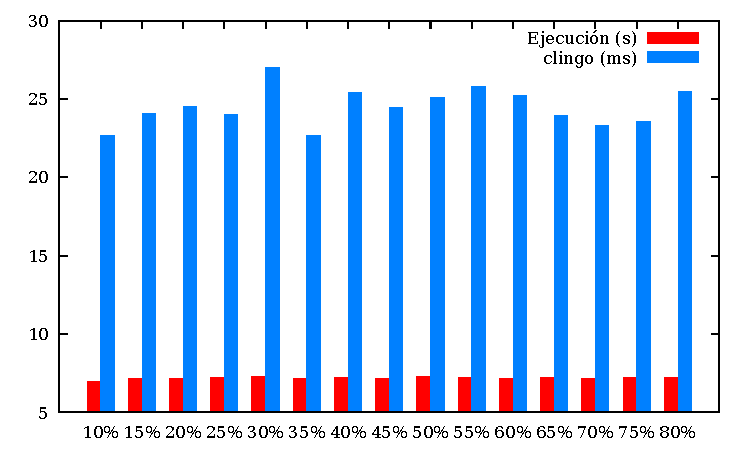
\includegraphics[width=.8\textwidth]{tables/land-size.pdf}
	\caption{Tiempos del \textit{benchmark} con diferentes porcentajes de tierra.}\label{fig:landresult}
\end{figure}

En la Tabla \ref{table:landresult} podemos ver los resultados de la realización de esta prueba de rendimiento ejecutando 25 ejecuciones cada una de las medidas, en donde se recoge el tiempo total de todas las ejecuciones, el tiempo total que ha usado clingo para obtener una solución y el tiempo medio de una ejecución. Por otra parte en la Figura \ref{fig:landresult} podemos ver una comparativa entre el tiempo medio entre ejecuciones y el tiempo medido arrojado por clingo. \\

En el caso de la segunda parte de la prueba se ha usado distintos porcentajes de cantidad de bioma que alcanza una isla, usando los mismos datos que para la prueba anterior. En la Tabla \ref{table:biomaresult} podemos ver los resultados de la realización de esta prueba de rendimiento ejecutando 25 ejecuciones cada una de las medidas, en donde se recoge el tiempo total de todas las ejecuciones, el tiempo total que ha usado clingo para obtener una solución y el tiempo medio de una ejecución. Por otra parte en la Figura \ref{fig:biomaresult} podemos ver una comparativa entre el tiempo medio entre ejecuciones y el tiempo medido arrojado por clingo. \\

\begin{table}[!h]
	\centering
	\begin{tabular}{ c c c }
		\bfseries{Porcentaje} & \bfseries{Total} & \bfseries{Ejecución} \\
		\hline
		10\% & 178 s & 7,12 s \\
		15\% & 180 s & 7,20 s \\
		20\% & 179 s & 7,16 s \\
		25\% & 178 s & 7,12 s \\
		30\% & 178 s & 7,12 s \\
		35\% & 179 s & 7,16 s \\
		40\% & 179 s & 7,16 s \\
		45\% & 213 s & 8,52 s \\
		50\% & 215 s & 8,60 s \\
		55\% & 216 s & 8.64 s \\
		60\% & 207 s & 8,28 s \\
		65\% & 192 s & 7,68 s \\
		70\% & 187 s & 7,48 s \\
		75\% & 208 s & 8,32 s \\
		80\% & 204 s & 8,16 s \\
		\hline
	\end{tabular}
	\caption{Resultado del \textit{benchmark} con diferentes porcentajes de tierra.}\label{table:biomaresult}
\end{table}

\begin{figure}[!h]
	\centering
	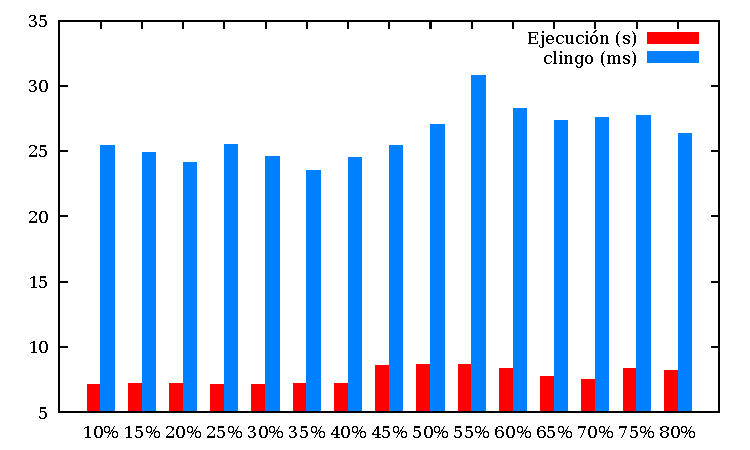
\includegraphics[width=0.8\textwidth]{tables/bioma-size.pdf}
	\caption{Tiempos del \textit{benchmark} con diferentes porcentajes de tierra.}\label{fig:biomaresult}
\end{figure}

Como se puede observar, en estas pruebas no se haya bastante diferencia al modificar uno de los valores, dando resultados muy similares entre si. Es por eso que se ha decidido combinar las dos pruebas en una sola para observar algún cambio efectivo. Esto se recoge en la Sección \ref{sec:pruebafinal}.

\section{Prueba mixta tierra/biomas}
\label{sec:pruebafinal}

En esta última prueba se ha tenido en cuenta los datos de la prueba relatada en la Sección \ref{sec:pruebatierrabiomas}, es decir, usando un mapa de 25x25 dividido en 5 cuadrantes de 5 celdas cada uno, con 4 islas totales y dejando el resto de variables con valores por defecto (tamaño de las cordilleras en 2 casillas, longitud de cordilleras en 3 casillas, 2 jugadores y 2 casillas de distancia mínima entre jugadores).

\begin{table}[!h]
	\centering
	\begin{tabular}{c|cccccc}
	 & 10\% & 15\% & 20\% & 25\% & 30\% & 35\% \\
	\hline
	10\% & 42 & 41 & 35 & 88 & 117 & 214 \\
	15\% & 41 & 37 & 36 & 88 & 133 & 247 \\
	20\% & 37 & 43 & 37 & 105 & 123 & 224 \\
	25\% & 29 & 51 & 43 & 92 & 123 & 220 \\
	30\% & 42 & 43 & 138 & 95 & - & - \\
	35\% & 41 & 40 & 38 & 90 & - & 241 \\
	40\% & 43 & 46 & 36 & -  & - & 217  \\
	45\% & 69 & 49 & 36 & 737 & - & 220 \\
	50\% & 100 & - & 1064 & - & - & - \\
	55\% & 55 & 956 & - & - & - & - \\
	60\% & 164 & 740 & - & - & - & - \\
	65\% & 97 & 838 & - & - & - & - \\
	\hline
	\end{tabular}
	\caption{Resultado del \textit{benchmark} con diferentes porcentajes de tierra (las columnas) y de biomas (las filas). Los tiempos totales son en segundos.}\label{table:finalresult}
\end{table}

Como se puede observar en los resultado mostrados en la Tabla \ref{table:finalresult}, en donde se han ejecutado 5 iteraciones por cada valor, el módulo de clingo obtiene resultados decentes cuando se establecen valores bajos para el porcentaje de tierra y de biomas, más el tiempo de ejecución se dispara en el momento de poner valores altos. Esto se debe a, como ya se ha comentado a lo largo de la memoria, el paradigma ASP puede llegar a tener en cuenta una gran combinación de datos y producirse una explosión combinatoria de soluciones, retardando en buena medida la procura de una solución.

	\section{Conclusiones}
	En este proyecto se construido una herramienta declarativa con la que elaborar, mediante programación lógica, nuevos escenarios para el videojuego Freeciv. Para ello se usó el paradigma de \textit{Answer Set Programming}, una variante de Programación Lógica de uso frecuente para la Representación del Conocimiento y la resolución de problemas. La principal ventaja de \textit{Answer Set Programming} para este caso fue la facilidad que otorgaba el uso de predicados simples a la hora de definir ciertas propiedades dentro de un escenario concreto, así como añadir directamente reglas de restricción para ciertos elementos del mapa bajo la forma de reglas de programación lógica. Esto proporcionó una gran flexibilidad, ya que con ello sólo se necesita realizar la especificación del problema sin importar el método de resolución que se aplicará. \\

También se ha reducido el problema que surge al tener en cuenta todas las reglas y restricciones del mapa, lo cual produce una explosión combinatoria de soluciones, y ocasionaba que el sistema tardase en encontrar. Para ello se ha separado el problemas de búsqueda del modelo declarativo en distintos módulos independientes: un generador de regiones, un módulo para rellenar las regiones, un generador de biomas, un módulo que define cordilleras, un módulo para definir las celdas de agua y por último un módulo para definir los puntos iniciales de los jugadores. \\

A pesar de todo esto, existen algunas limitaciones de cara la finalización de este proyecto, las cuales pueden ser resueltas en un futuro inmediato:

\begin{itemize}
	\item El sistema no tiene en cuenta todos los elementos que proporciona el videojuego, por lo que no soporta actualmente la generación de ríos, ni la generación de recursos ni la generación de puntos de inicio para bárbaros o aldeas perdidas. Esto se podría solucionar añadiendo nuevos módulos a la generación del mismo.
	\item El sistema presenta graves problemas de eficiencia a la hora de generar grandes porciones de mapas, mermando la funcionalidad de la herramienta. Esto se puede observar en la Sección \ref{evaluation}, en donde había problemas con mapas mayores de 45x45 celdas en cuanto a tiempo de ejecución. Esto se podría resolver intentando pulir las reglas actuales de los módulos o replanteando la forma en la que se han definido, en algunos casos dividiendo más para reducir la carga de estos.
\end{itemize}

Para finalizar, se puede marcar una serie de líneas, tanto para solucionar y mejorar el sistema propuesto como para ampliar y extender las funcionalidades actuales de cara a largo plazo:

\begin{itemize}
	\item Mejorar la interfaz gráfica, incluyendo distintos elementos gráficos con los que manejar de forma más efectiva el mapa, como puede ser herramientas para ampliar y disminuir el mapa, mover el mapa o marcar de forma más visual el tipo de terreno marcar.
	\item Indicar de forma más visual restricciones en el mapa, así como zonas que tendrá en cuenta el generador para completar. Estas zonas incluso pueden tener restricciones de que piezas no poner o preferencias de los tipos de terrenos a generar.
	\item Publicar y anunciar la herramienta para tener una buena base de usuarios que puedan producir un \textit{feedback} del uso y características de la misma.
	\item Añadir a la base de conocimiento estilos personalizados, ya sea incluyéndolos dentro de las reglas o importándolos como perfiles. Estos permitirían que un usuario pueda tener preferencias de cara a la generación (que no le guste generar cordilleras cerca del agua, que los usuarios estén lo más cercano a bosques o recursos, etc).
\end{itemize}

	\begin{frame}
		\vbox{}
		\vspace{0.25em}
		\begin{centering}
			{\usebeamercolor[fg]{titlegraphic}\inserttitlegraphic\par}
			\vspace{0.5em}
			\begin{beamercolorbox}[sep=8pt,center,rounded=true]{title}
				\usebeamerfont{title}\inserttitle\par%
				\ifx\insertsubtitle\@empty%
				\else%
				\vspace{0.25em}
				{\usebeamerfont{subtitle}\usebeamercolor[fg]{subtitle}\insertsubtitle\par}%
				\fi%     
			\end{beamercolorbox}%
			\vfill
			\begin{beamercolorbox}[sep=8pt,center]{author}
				\usebeamerfont{author}\insertauthor
			\end{beamercolorbox}
			\vspace{0.5em}
			{\Large\textcolor{UDCpink}{¡Gracias por vuestra atención!}\par}
			\vspace{0.5em}
			\begin{beamercolorbox}[sep=8pt,center]{institute}
				\usebeamerfont{institute}\insertinstitute
			\end{beamercolorbox}
			\begin{beamercolorbox}[sep=8pt,right]{date}
				\itshape\usebeamerfont{date}\insertdate
			\end{beamercolorbox}
		\end{centering}
		\vspace{0.25em}
	\end{frame}

	\begin{frame}
	\frametitle{Ejemplo de la biblioteca de Clingo}
	
	\begin{block}{Añadir restricciones al programa}
		\ttfamily \footnotesize
		
		\#script(lua)
		
		\textbf{function} main(prog)
		
		\hspace{2em} \textit{\textendash\textendash Genero las regiones}
		
		\hspace{2em} \textbf{for} i = 0, c\_regions-1 \textbf{do}
		
		\hspace{4em} \textit{\textendash\textendash Hace grounding del programa lógico}
		
		\hspace{4em} prog:ground(\{\{''base'', \{\}\}, \{''generate'', \{i\}\}\})
		
		\hspace{4em} \textit{\textendash\textendash Obtengo un manejador de la solución}
		
		\hspace{4em} handle = prog:solve({yield=true})
		
		\vspace{1em}
		
		\hspace{4em} \textbf{local} restrictions = '' ''
		
		\hspace{4em} \textit{\textendash\textendash Recorre los modelos de la solución}
		
		\hspace{4em} \textbf{for} model \textbf{in} handle:iter() \textbf{do}
		
		\hspace{6em} \textit{\textendash\textendash Añado las restricciones}
		
		\hspace{6em} \textbf{if} \#restrictions \textasciitilde{}= 0 \textbf{then}
		
		\hspace{8em} prog1:load(''resources/restrictions.lp'')
		
		\hspace{6em} \textbf{end}
		
		\hspace{6em} ...
		
	\end{block}
	\end{frame}
	
	\begin{frame}
	\frametitle{Ejemplo de la biblioteca de Clingo}
	
	\begin{block}{Añadir restricciones al programa}
	\ttfamily \footnotesize
	
	\hspace{6em} \textbf{for} m \textbf{in} handle:iter() \textbf{do}
	
	\hspace{8em} \textbf{for} row\_str, col\_str, contain \textbf{in} string.gmatch(tostring(model), 	''cell\%(p\%((\%d+),(\%d+)\%),(\%l+)\%)'') \textbf{do}
	
	\hspace{10em} \textbf{if} contain == "l"  \textbf{then}
	
	\hspace{12em} lands = lands .. '' land(p(''..row\_str..'',''..col\_str..'')).''
	
	\hspace{12em} restrictions = restrictions .. check\_restrictions(row, col, i)
	
	\hspace{10em} \textbf{end}
	
	\hspace{8em} \textbf{end}
	
	\vspace{1em}
	
	\hspace{8em} df = io.open(''resources/restrictions.lp'', ''w+'')
	
	\hspace{8em} df:write(restrictions)
	
	\hspace{8em} df:flush()
	
	\hspace{8em} df:close()
	
	\hspace{6em} \textbf{end}
	
	\hspace{4em} \textbf{end}
	
	\hspace{2em} \textbf{end}
	
	\textbf{end}
	
	\#end.
	\end{block}
	\end{frame}

	\begin{frame}
	\frametitle{Ejecución del módulo Clingo}
	
	\centering
	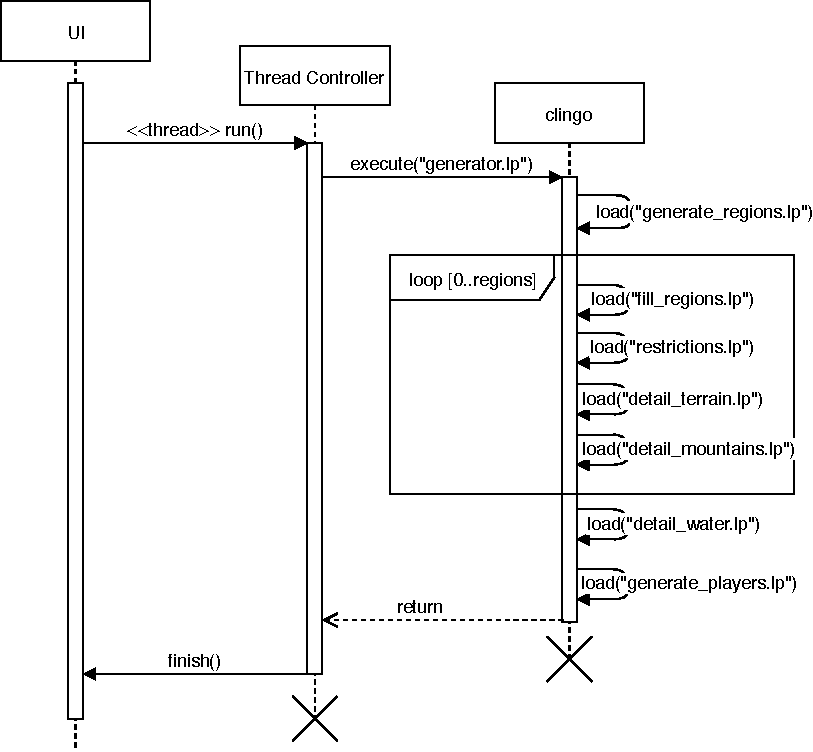
\includegraphics[width=0.6\textwidth]{images/diagrama-secuencia.pdf}
	
	\end{frame}

\end{document}